%!TEX root =  tfg.tex
\chapter{Concepts théoriques et méthodologiques}

\begin{quotation}[Novelist]{Ernest Hemingway (1899--1961)}
The good parts of a book may be only something a writer is lucky enough to overhear or it may be the wreck of his whole damn life -- and one is as good as the other.
\end{quotation}

\begin{abstract}
Resumen de lo que va a ocurrir en el capítulo. ¿Cuál es el objetivo que tenemos con este capítulo?
\end{abstract}

\section{Présentation du RGPD}
\subsection{Origines}
Le Règlement Général sur la Protection des données en abrégé RGPD est une loi qui concerne la protection des données personnelles des utilisateurs habitants d’un pays de l’Union Européenne. Il vient remplacer la Directive sur la protection des données personnelles adoptée en 1995. Le RGPD a été finalement adopté par le Parlement Européen le 14 Avril 2016 ; ses dispositions sont applicables dans tous les états membres de l’Union Européenne à compter du 25 Mai 2018.

Il est important de noter que le RGPD s’applique [1]:
\begin{itemize}
   \item[•] Aux entreprises ou entités qui traitent des données à caractère personnel dans le cadre des activités de l’une de leurs filiales établie au sein de l’UE, indépendamment de l’endroit où sont traitées les données ;
   \item[•] Aux entreprises établies en dehors de l’UE qui proposent des biens ou services (payants ou gratuits), ou surveillent le comportement des personnes dans l’UE.
\end{itemize}

\subsection{Objectifs}
Le RGPD a les différents objectifs suivants [2] :
\begin{itemize}
   \item[•] Renforcer le droit des personnes;
   \item[•] Responsabiliser les acteurs traitants les données;
   \item[•] Crédibiliser la régulation.
\end{itemize}
L’on peut donc retenir que les principaux objectifs du RGPD sont d’accroître à la fois la protection des personnes dont les données à caractère personnel sont traitées et de responsabiliser les acteurs de ce traitement. 
\subsection{Principes}
Le type et la quantité de données à caractère personnel qu’une entreprise/organisation peut traiter dépendent de la raison pour laquelle elles sont traitées et le but dans lequel elles le sont. Ainsi, l’entreprise/organisation doit respecter un certain nombre de principes [3] :
\begin{itemize}
   \item[•] Les données personnelles doivent être traitées de manière licite et transparente : \textbf{licéité, loyauté et transparence};
   \item[•] Il doit y avoir des finalités précises pour traiter des données et l’entreprise/organisation doit indiquer ces finalités aux personnes dont les données sont collectées : \textbf{limitation des finalités};
   \item[•] \textbf{Minimisation des données:} l’entreprise ne peut traiter que les données personnelles qui sont nécessaires pour atteindre ces finalités ;
   \item[•] \textbf{Exactitude:} L’entreprise doit s’assurer que les données personnelles collectées sont exactes et mises à jour ;
   \item[•] L’entreprise ne peut utiliser les données collectées pour d’autres finalités qui ne sont pas compatibles avec celles pour lesquelles elles ont été initialement collectées ;
   \item[•] \textbf{Limitation de la conservation:} les données collectées ne doivent pas être gardées plus longtemps que nécessaires ;
   \item[•] \textbf{Responsabilité:} l’on doit pouvoir démontrer la conformité de l’entreprise avec le RGPD, mener une analyse d’impact relative à la protection des données, …
   \item[•] \textbf{Limitation des transferts:} pas de transfert de données d’un territoire à l’autre à moins que ce pays ou territoire assure un niveau de protection adéquat des droits et libertés des propriétaires des données ;
   \item[•] \textbf{Intégrité et confidentialité:} l’entreprise doit mettre en place des mesures techniques et organisationnelles afin de garantir la sécurité des données collectées.
\end{itemize}
\subsection{Sanctions en cas de non-conformité}
En cas de non-respect du RGPD, l’entreprise/organisation s’expose aux sanctions suivantes :
\begin{itemize}
  \item[•] \textbf{20 millions d'Euros} pour les PME;
  \item[•] Jusqu’à plusieurs milliards d’euros pour les grands groupes, il s’agit plus précisément de \textbf{4\% du chiffre d'affaires} global du groupe.
\end{itemize}

\section{Méthodologie}

L’information est d’une importance capitale dans une entreprise. Pouvoir tracer le cycle de vie de l’information est une activité incontournable afin de protéger et sécuriser celle-ci.

Afin d’aboutir à une solution de classification des données de l’entreprise, nous avons suivi un ensemble d’étapes [4].

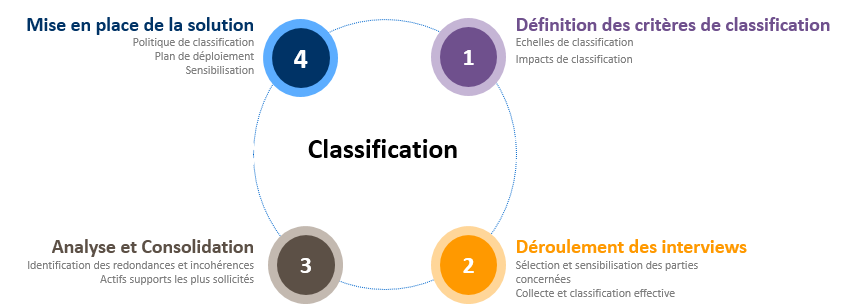
\includegraphics{methodologie.png}

\begin{enumerate}
   \item \textbf{Définition des critères de classification des données}
   \begin{enumerate}
     \item \textbf{Echelles de classification}
     
     Le but de la classification des données est de garantir la sécurité des données sans entraver la fluidité de l’information et des processus de l’entreprise. Pour se faire, il est important de définir des échelles de classification se basant sur les 3 concepts de la sécurité : la confidentialité, l’intégrité et la disponibilité.
     \item \textbf{Impacts de classification}
     
     En entreprise, les informations sont identifiées suivants des niveaux d’exposition au risque et de granularité (groupes d’information, données élémentaires, …). Ainsi l’impact associé en cas de divulgation ou d’altération sera fonction de ces niveaux. Les impacts de la perte de confidentialité, d’intégrité et de disponibilité de l’information sont intriqués.  Ces impacts peuvent présenter pour l’entreprise des défis pour sa conformité légale, réglementaire et contractuelle, ses opérations quotidiennes, sa réputation ou ses finances. Nous avons donc choisi de catégoriser les impacts ainsi que  montre la figure suivante : Voir annexe 1.
   \end{enumerate}
   \item \textbf{Déroulement des interviews}
   \begin{enumerate}
       \item \textbf{Sélection et Sensibilisation des partis concernés}
       
       Pour mener à bien cette activité de classification, il est important de choisir les interlocuteurs compétents et qualifiés, ayant autorité de décision sur les processus et informations pour lesquels ils sont sollicités. Une étape de sensibilisation afin de préparer l’interlocuteur à fournir les informations pertinentes pour une bonne classification.
       \item \textbf{Collecte et classification des informations}
       
       Les informations ont été collectées à travers des interviews des interlocuteurs choisis. 
       
        La première étape consiste à identifier tous les processus de l’entreprise ainsi et surtout le flux des informations essentielles le long du processus considéré. Ensuite pour chaque activité ou processus, nous allons cartographier les éléments récoltés suivant certains critères. Cette étape terminée nous obtenons notre classification des données.

   \end{enumerate}
   \item \textbf{Analyse et consolidation des informations collectées}
   
   Dans cette étape, nous allons épurer l’ensemble des paramètres récoltés, identifier les éléments redondants et d’éventuelles incohérences, aussi nous allons mettre en évidence les actifs supports les plus sollicités au sein de l’entreprise.
   
L’analyse nous permettra également de faire ressortir les risques opérationnels apportés par la mise en place des mesures de sécurité ; l’on devra donc ici identifier les mesures adéquates et proportionnées, alignée sur les niveaux de classification pertinents, et veiller à leur mise en œuvre effective.

   \item \textbf{Mise en place de la solution de classification}
   \begin{enumerate}
       \item \textbf{Politique de classification}
       
       Une fois collectés, classifiés et analysés nous devons formaliser dans une politique de classification, les règles et mesures de sécurité à appliquer pour assurer leur protection adéquate. Cette politique énonce les règles de classification et propose une démarche de mise en œuvre pragmatique des mesures de protection pour chaque niveau de classification et à chaque étape du cycle de vie de l’information.
       \begin{itemize}
           \item[-] Détermination des paramètres du déploiement
           \begin{itemize}
               \item[o] Responsable des mesures de sécurité identifiées;
               \item[o] Echéances de déploiement;
               \item[o] Ressources nécessaires.
           \end{itemize}
           \item[-] Détermination des rôles et responsabilités minimum pour la classification des données
           \begin{itemize}
               \item[o] Les propriétaires de l'information;
               \item[o] Le responsable du suivi et du maintien de la planification;
               \item[o] La liste des partis prenantes impliqués dans la revue de la classification.
           \end{itemize}
       \end{itemize}
       \item \textbf{Plan de déploiement}
       \item \textbf{Sensibilisation}
   \end{enumerate}
 \end{enumerate}